\subsection{Statistique descriptive en 2D}


\subsubsection{Covariance}

\begin{center}
	\begin{tabular}{ccc}
		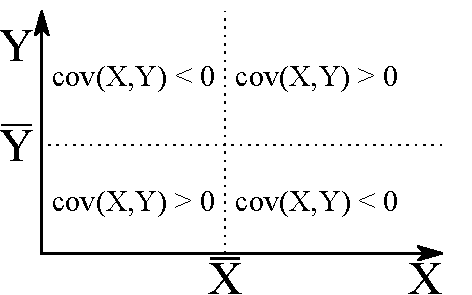
\includegraphics[width=0.3\textwidth]{images/covariance-all.pdf}&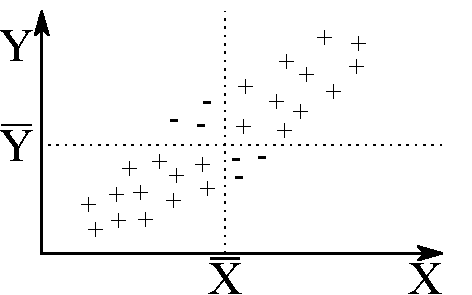
\includegraphics[width=0.3\textwidth]{images/covariance-positive.pdf}&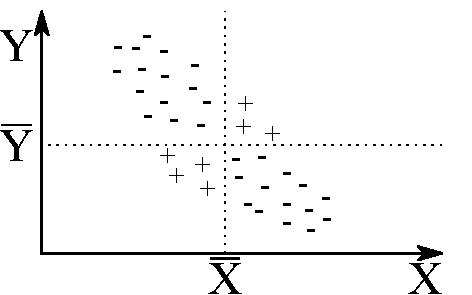
\includegraphics[width=0.3\textwidth]{images/covariance-negative.pdf}\\
		Allure générale&$n_{11}>0$&$n_{11}<0$
	\end{tabular}
\end{center}





\paragraph{La covariance $|m_{11}| \leq s_1s_2$}

La covariance est le moment d'ordre (1,1):

$$m_{11}=\frac{1}{n} \sum_{i=1}^{p} \sum_{j=1}^{q} n_{ij} (x_i-\bar{x})(y_j-\bar{y})$$

\begin{align*}
	\alpha  &= \frac{1}{n} \sum_{i=1}^{p} \sum_{j=1}^{q} n_{ij} \underbrace{ ((x_i-\bar{x})(y_j-\bar{y}))^2 }_\text{$^2$ car toujours $\geq 0$} \\
	        &= \frac{1}{n} \sum_{i=1}^{p} \sum_{j=1}^{q} n_{ij} (u^2(x_i-\bar{x})^2 + 2a(x_i-\bar{x})(y_j-\bar{y})+(y_j-\bar{y})^2)\\
	        &= u^2s_1^2+2u\ m_{11}+s_2^2
\end{align*}

Équation du second degré, on calcule son $\Delta$ :
\begin{align*}
\Delta &\leq 0\\
m_{11}^2-s_1^2s_2^2 &\leq 0\\
m_{11}^2 &\leq s_1^2s_2^2\\
|m_{11}| &\leq s_1s_2
\end{align*}





\paragraph{La covariance maximale $|m_{11}| = s_1s_2$}

La valeur absolue de la covariance est maximale et vaut $|m_{11}| = s_1s_2$.

Si les points observés se trouvent sur une droite $ax+bx+c=0$, on a $ax_i+by_i+c=0$.

On multiplie par $\frac{n_{ij}}{n}$ et on somme sur $ij$.

\begin{align*}
0  &= \sum_{i=1}^{p} \sum_{j=1}^{q} \frac{n_{ij}}{n}(ax_i+by_j+c) \\
   &= a \frac{1}{n} \sum_{i=1}^{p} \sum_{j=1}^{q}n_{ij}x_i + b \frac{1}{n} \sum_{i=1}^{p} \sum_{j=1}^{q}n_{ij}y_j + c \frac{1}{n} \sum_{i=1}^{p} \sum_{j=1}^{q}n_{ij}\\
   &= a\bar{x}+b\bar{y}+c\\
\intertext{On soustrait $ax_i+by_j+c=0$ par $a\bar{x}+b\bar{y}+c = 0$.}
   &= a(x_i-\bar{x})+b(y_j+\bar{y})\\
\intertext{On utilise $u_0=\frac{a}{b}$}
   &= u_0b(x_i-\bar{x})+\frac{a}{u_0}(y_j-\bar{y})\\
   &= u_0b(x_i-\bar{x})+\frac{u_0b}{u_0}(y_j-\bar{y})\\
   &= u_0(x_i-\bar{x})+(y_j-\bar{y})
\end{align*}

L'équation a la même forme que $\alpha$, du coup...
\begin{align*}
0  &= \Delta\\
        &= m_{11}^2-s_1^2s_2^2\\
m_{11}^2 &= s_1^2s_2^2\\
|m_{11}| &= s_1s_2
\end{align*}




\subsubsection{Le coefficient de corrélation}
$$\boxed{r=\frac{m_{11}}{s_1s_2}}$$







\newpage
\subsubsection{Les droites de régression}

\begin{center}
	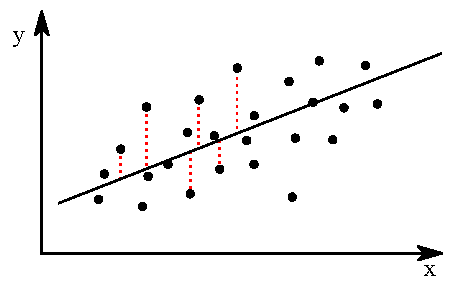
\includegraphics[width=0.3\textwidth]{images/droite_de_regression.pdf}
\end{center}
La droite de régression de y en x est la droite qui minimise la somme des carrés des écarts (parallèles à l'axe y) des points observés à cette droite.
$$\boxed{g(a,b) = \sum_{i=1}^{p} \sum_{j=1}^{q} n_{ij} (y_j - a\ x_i - b)^2}$$


\textbf{Dérivée par rapport à $a$.}
\begin{align*}
0 &= \left.g(a,b)\right|_a\\
  &= \sum_{i=1}^{p} \sum_{j=1}^{q} n_{ij}\ 2(y_j - a\ x_i-b)(-x_i)\\
  &= \sum_{i=1}^{p} \sum_{j=1}^{q} -2n_{ij}\ x_i(y_j - a\ x_i - b)\\
  &= \sum_{i=1}^{p} \sum_{j=1}^{q} n_{ij}\ x_i(-y_j + a\ x_i + b)\\
  &= \sum_{i=1}^{p} \sum_{j=1}^{q} -n_{ij}\ x_i\ y_j + \sum_{i=1}^{p} \sum_{j=1}^{q} n_{ij}\ a\ x_i^2 + \sum_{i=1}^{p} \sum_{j=1}^{q} n_{ij}\ b\ x_i\\
  &= -1 \sum_{i=1}^{p} \sum_{j=1}^{q} n_{ij}\ x_i\ y_j + a \sum_{i=1}^{p} \sum_{j=1}^{q} n_{ij}\ x_i^2 + b \sum_{i=1}^{p} \sum_{j=1}^{q} n_{ij}\ x_i\\
  \sum_{i=1}^{p} \sum_{j=1}^{q} n_{ij}\ x_i\ y_j  &= \underbrace{a \sum_{i=1}^{p} \sum_{j=1}^{q} n_{ij}\ x_i^2 + b \sum_{i=1}^{p} \sum_{j=1}^{q} n_{ij}\ x_i}_\text{Il n'existe aucun terme en $j$}\\
\sum_{i=1}^{p} \sum_{j=1}^{q} n_{ij}\ x_i\ y_j  &= \overbrace{a \sum_{i=1}^{p} n_{i.}\ x_i^2 + b \sum_{i=1}^{p} n_{i.}\ x_i}^\text{Donc on peut supprimer la somme $\sum_{j=1}^{q}$}
\end{align*}


$$\boxed{\sum_{i=1}^{p} \sum_{j=1}^{q} n_{ij}\ x_i\ y_j = a \sum_{i=1}^{p} n_{i.}\ x_i^2 + b \sum_{i=1}^{p} n_{i.}\ x_i}$$


\textbf{Dérivée par rapport à $b$.}
\begin{align*}
0 &= \left.g(a,b)\right|_b\\
  &= \sum_{i=1}^{p} \sum_{j=1}^{q} n_{ij}\ 2(y_j - a\ x_i-b)(-1)\\
  &= \sum_{i=1}^{p} \sum_{j=1}^{q} -2n_{ij}(y_j - a\ x_i - b)\\
  &= \sum_{i=1}^{p} \sum_{j=1}^{q} n_{ij}(-y_j + a\ x_i + b)\\
  &= \sum_{i=1}^{p} \sum_{j=1}^{q} -n_{ij}\ y_j + \sum_{i=1}^{p} \sum_{j=1}^{q} n_{ij}\ a\ x_i + \sum_{i=1}^{p} \sum_{j=1}^{q} n_{ij}\ b\\
  &= -1 \sum_{i=1}^{p} \sum_{j=1}^{q} n_{ij}\ y_j + a \sum_{i=1}^{p} \sum_{j=1}^{q} n_{ij}\ x_i + b \sum_{i=1}^{p} \sum_{j=1}^{q} n_{ij}\\
\sum_{i=1}^{p} \sum_{j=1}^{q} n_{ij}\ y_j &= a \sum_{i=1}^{p} \sum_{j=1}^{q} n_{ij}\ x_i + b \sum_{i=1}^{p} \sum_{j=1}^{q} n_{ij}\\
n\ \bar{y} &= a\ n\ \bar{x} + b\ n
\end{align*}

$$\boxed{n\ \bar{y} = a\ n\ \bar{x} + b\ n}$$


On a obtenu ces deux réponses
\begin{equation*}
\left\{
\begin{aligned}
	\sum_{i=1}^{p} \sum_{j=1}^{q} n_{ij}\ x_i\ y_j &= a \sum_{i=1}^{p} n_{i.}\ x_i^2 + b \sum_{i=1}^{p} n_{i.}\ x_i &(1)\\
	n\ \bar{y} &= a\ n\ \bar{x} + b\ n &(2)
\end{aligned}
\right.
\end{equation*}


\begin{align*}
	\bar{x}\ (2) &: n\ \bar{y}\ \bar{n} = a\ n\ \bar{x}^2 + b\ n\ \bar{n}\\
	(1) - \bar{x}\ (2) &: 
\end{align*}